%!TEX root = ../main.tex

Bitcoin currently achieves about 7 transactions per second. 
Also, to be sure that a transaction is included, clients wait for 6 blocks, which takes 
on average 1 hour.
In this chapter we discuss different approaches to increase this throughput and reduce confirmation latency.

\begin{definition} \textbf{Throughput} of a blockchain is the maximum number of transaction that can be included in the chain per second.
\end{definition}

\begin{definition} \textbf{Comfirmation latency} of a blockchain is the time it takes from when a transaction is first included in a block, until it can be considered confirmed, and a client can be sure that it will not be removed from the chain.
\end{definition}

\section{Blocksize and block interval}
To increase this, it was heavily discussed, wether the blocksize should be increased, or block frequency can be reduced.

\begin{definition} A change in maximum blocksize or target block interval is called a \emph{reparametrization}.
\end{definition}

Research, (see resources.md) has suggested that network latency grows linearly with blocksize.
\begin{lem} 
	A reparametrization that increases blocksize will result in higher network latency and thus in an increased fork probability.
\end{lem}
\begin{proof}
Theorem~\ref{thm:fork} says that increased network latency results in higher fork probability.	
\end{proof}

\begin{lem}
	A reparametrization that decreases target block interval causes an increased fork probability.
\end{lem}
\begin{proof}
A reduced target block interval,~i.e., less than the current 10~min value, will result in an increased probability that a block is found within a second ($p$ in Theorem~\ref{thm:fork}).
\end{proof}

An increased fork probability creates the following \textbf{problems}:
\begin{enumerate}
	\item \textbf{Security} Forks among the honest miners make selfish mining more efficient and make a 51\% attack easier. 
	\item \textbf{Centralization} Forks are bad for small miners, since they are likely to loose their mining reward in a fork. Thus frequent forks favor centralization and the formation of larger mining pools.
\end{enumerate}

To measure these, the following metrics exist: See [Bitcoin NG] for definition and evaluation.
\begin{definition}
\textbf{Mining power utilization} is the number of blocks in the longest chain, devided by the total number of blocks created. 
\end{definition}
Mining power utilization is related to the security problem above.

\begin{definition}
	\textbf{Fairness} given the fraction with the largest mining power (or one such fraction). Fairness is defined as the percentage of block in the longest chain, not published by this party, divided by the percentage of blocks not mined by this party, relative to all blocks, including forks.
\end{definition}

\subsection{Ghost}
GHOST is a proposal to avoid the security problem (1.) that may arise with more frequent forks, namely increased vulnerability to selfish mining and double spend attacks. This is especially relevant to maintain security after reparametrization for increased throughput.

\begin{definition} The \emph{Greedy heaviest-observed subtree (GHOST)} rule says, instead of selecting the longest chain the root of the subtree containing most blocks should be selected.	
\end{definition}

\begin{note}
	\begin{itemize}
		\item As long as only a single fork exists, the GHOST rule is identical with the longest chain rule.
		\item In a selfish-mining attack the attackers chain will not contain any forks, since only a single node/agent is trying to extend it. The chain build by honest nodes may show additional forks. Using the GHOST rule, these forks do not give an advantage to the attacker.
		\item Using network attacks the attacker may cause forks on the honest chain. Using the GHOST rule, these attacks have no impact on the probability of a successful attack.
	\end{itemize}
\end{note}

\subsection{Inclusive chains and uncles}
Inclusive chains are a possibility to address Problem 2, \textbf{Centralization}.
An increased fork probability may result in many blocks being discarded. This results in miners not getting their block rewards. It provides an incentive for miners/nodes to form larger groups, rather than mine individually. 
This is true also when using the GHOST rule.

\begin{definition} The published blocks, both on the longest chain and in other forks, build a \emph{tree}, routed at the genesis block.
The \emph{previous block hash} $h_{-1}$ pointers point to the parent of a block.
\end{definition}
\begin{definition}
	In an \emph{inclusive} blockchain, instead of just including the hash of the parent, a block $b_{new}$ can include hashes of another block $b$, if:
	\begin{itemize}
		\item $b$ is not an ancestor of $b_{new}$
		\item the depth of $b$ ($d_b$) (i.e. distance from the genesis block) is less than the depth of $b_{new}$ ($d_{new}$).
	\end{itemize}
	Blocks included as additional ancestors are called \emph{uncles.}
\end{definition}

\begin{definition}
In an inclusive blockchain, blocks may receive an \textbf{uncle reward} and \textbf{nephew reward}.
	\begin{itemize}
		\item A block $b$ included as uncle in $b_{new}$ receives a fraction of the block-reward, the \textbf{uncle reward}. The fraction reduces with the distance between $b$ and $b_{new}$,~i.e. $d_{new}-d_{b}$.
		\item A block $b_{new}$ receives a small reward (\textbf{nephew reward}) for every uncle it includes.
	\end{itemize}
\end{definition}

\begin{example}
Ethereum uses uncle blocks. An uncle $b$ is rewarded $1-\frac{(d_{new}-d_b)}{7}$ of the block reward. Thus uncles that are more than 6 blocks behind are not rewarded.

For including an uncle a block creator is rewarded $\frac{1}{32}$ of a block reward.

Ethereum also requires that an uncle  is a child to one of the ancestors of the nephew. Thus, on longer forks, only the first block can be an uncle.
\end{example}

\begin{note}
Security and incentives:
\begin{itemize}
	\item The possibility to receive a block reward, being not included in the main chain, reduces the urge to form larger mining groups (pools).
	\item The reward an uncle receives plus the reward for including an uncle is less than the block reward. This should incentivize nodes to try and extend the main chain.
	\item The reward for uncles is reduced over distance. This discourages keeping blocks secret. 
\end{itemize}
\end{note}


\begin{theorem} 
In an inclusive blockchain, the selfish mining attack becomes profitable at a lower $\alpha$ threshold than without inclusive mining.

This can be leveraged to some extend, if the difficulty is adjusted not based on the frequency of blocks on the main chain, but based on the frequency of blocks on the main chain, and uncles.
\end{theorem}
\begin{proof} See \href{https://arxiv.org/pdf/1901.04620.pdf}{Selfish Mining in Ethereum} 
	\begin{figure}[H]
		\centering
		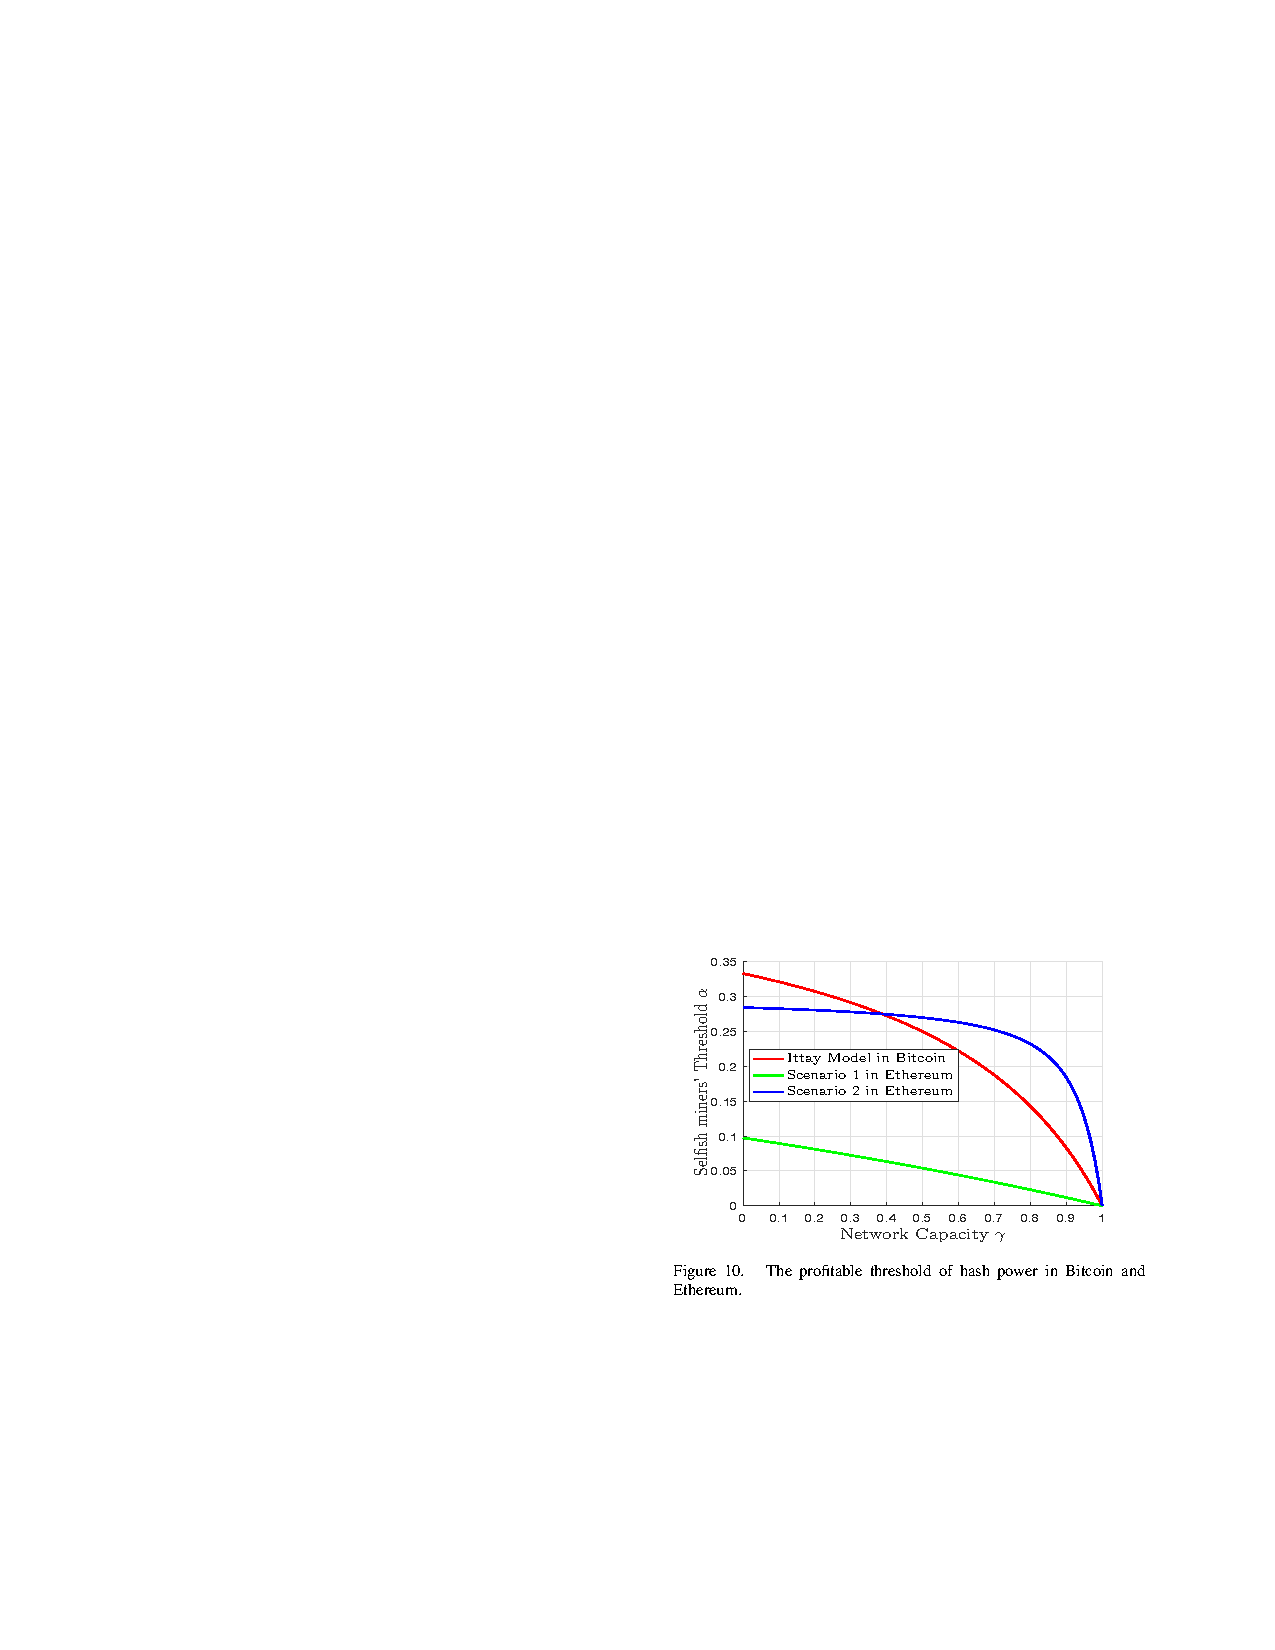
\includegraphics{fig/inclusive-selfish-mining}
	\end{figure}
	In the above figure from [Selfish Mining in Ethereum, ICDCS'19] Scenario 1 is where block difficulty is only adjusted based on the new blocks on the main chain.
	Scenario 2 adjusts difficulty based on creation of blocks and uncle blocks.
	
\end{proof}

\section{Uncles for scaling}
In Ethereum, the transactions included in uncle blocks are not applied. However, it is possible to also apply these transactions.

\begin{theorem}
	\label{thm:uncleorder}
It is possible to define a deterministic order on all blocks in a chain and all uncles in a chain, such that the order extends when the chain is extended.
This allows to execute transactions that are included in the uncle blocks, but not in the main chain.
\end{theorem}

\begin{proof}
	The order is done based on the following principles, from highest to lowest priority:
	\begin{itemize}
		\item Ancestors of $b_{new}$ are ordered before uncles of $b_{new}$.
		\item Uncles of $b_{new}$ are ordered before $b_{new}$.
		\item Uncles are ordered according to their depth.
		\item At the same depth, uncles are ordered according to their hash.
	\end{itemize}
\end{proof}

\begin{note}
Inclusive blockchains have the following effect on scalability:
\begin{itemize}
	\item If uncle blocks include transactions that are not included or conflicting with the main chain this can further increase scalability. Execution of transaction in uncles is not implemented in Ethereum.
	\item Given execution of transactions in uncles, it is difficult how to incentivize different blocks in a fork, to include different transactions.
	\item It is possible to extend inclusive blockchains to allow uncles that are not children of ancestors in the current main chain. Theorem~\ref{thm:uncleorder} still holds, but becomes more complex.
\end{itemize}
\end{note}

\section{Bitcoin NG}
See resources.md on course info for Video, slides, paper, ...

\begin{definition} Bitcoin-NG differentiates between \emph{Keyblocks} and \emph{Microblocks}. 
	\begin{description}
		\item[Keyblocks] Include a proof of work. No transactions, a public key, and the hash of the last Key- or Microblock.
		\item[Microblocks] Include no PoW but transactions, a previous block hash, and a signature matching public key from last KeyBlock.
	\end{description}

	\noindent
	\textbf{Fork resolutions} Longest chain rule (or GHOST) is used but only looks at the Keyblocks.
	\textbf{Fee distribution} Fees are distribution between the creator of the microblock (40\%) and the creator of the next Keyblock (60\%).
\end{definition}

\begin{note} 
	(Bitcoin-NG)\newline
	
	
	\begin{itemize}
		\item Security and fork probability (keyblocks) is decoupled from throughput and transaction rate (microblocks).
		\item The distribution of fees (40/60) ensures that it is better to reference the latest microblock, rather than keeping the transactions for your own microblocks. Also significant incentive for actually publishing microblocks.
	\end{itemize}

\noindent	
\textbf{Problem}
	\begin{itemize}
		\item Since Bitcoin-NG relies on a leader, progress can be reduced through leader failure. A single leader failure will not be a problem, but if an attacker causes multiple leaders to fail, e.g. by a DDOS (Distributed denial of service) attack, transaction throughput may be significantly reduced.
	\end{itemize}
\end{note}

\begin{example}
To understand the choice of 40\%, 60\% fee distribution, consider the example in Figure~\ref{fig:bitng-1}. Squares represent key blocks, while circles represent microblocks. 

In Figure~\ref{fig:bitng-1} the minor of the red block gets 60\% of the fees from the yellow transactions from microblock $b_0'$.

If he instead mines on top of $b_0$, he can himself publish a microblock including the yellow transactions. This is shown in Figure~\ref{fig:bitng-2}.
In this case the red minor receives 40\% of the fees from yellow transactions. 
Additionally, if the red minor has a fraction of the mining power equal to $\alpha$, he has a probability $\alpha$ to mine key-block $b_2$ and get additional 60\% of the yellow fees. 
If $\alpha<0.33$ then $0.4+\alpha\cdot 0.6 < 0.6$. Thus the red minor will try to extend $b_0'$.

Similarly, if the blue minor does not publish block $b_0'$ but instead hopes to publish $b_2$ in Figure~\ref{fig:bitng-2}, his expected fraction of the yellow fees is $\beta\cdot 0.6 <0.4$. Thus for a hashing fraction $\beta<0.33$ it is better to publish $b_0'$.
	\begin{figure}[h]
		\centering
		%!TEX root = ../main.tex

\begin{tikzpicture}
	[block/.style={rectangle,draw,thick, minimum size=1cm},
	mblock/.style={circle,draw,thick, minimum size=1cm},
	dblock/.style={block, dashed},
	noblock/.style={block, white},
	prev/.style={draw, -latex, thick}, 
	dprev/.style={prev, dashed},
	just/.style={-latex, double, thick, red},
	justarc/.style={out=135, in=45},
	interval/.style={|-|, dashed, thick},
	node distance =.5cm and 1cm]
	\node(b0)[block, draw=blue]{$b_0$};
	\node(b1)[mblock, right=of b0, fill=yellow]{$b_0'$};
	\draw[prev](b1) -- (b0);
	\node(b2)[block, right=of b1, draw=red]{$b_1$};
	\draw[prev](b2) -- (b1);
	
	
	
\end{tikzpicture}
		\caption{Red miner gets 60\% of yellow transactions.}
		\label{fig:bitng-1}
	\end{figure}
	\begin{figure}[h]
		\centering
		%!TEX root = ../main.tex

\begin{tikzpicture}
	[block/.style={rectangle,draw,thick, minimum size=1cm},
	mblock/.style={circle,draw,thick, minimum size=1cm},
	dblock/.style={block, dashed},
	noblock/.style={block, white},
	prev/.style={draw, -latex, thick}, 
	dprev/.style={prev, dashed},
	just/.style={-latex, double, thick, red},
	justarc/.style={out=135, in=45},
	interval/.style={|-|, dashed, thick},
	node distance =.5cm and 1cm]
	\node(b0)[block,draw=blue]{$b_0$};
	\node(b1)[block, right=of b0, draw=red]{$b_1$};
	\draw[prev](b1) -- (b0);
	\node(b2)[mblock, right=of b1, fill=yellow]{$b_1'$};
	\draw[prev](b2) -- (b1);
	\node(b3)[dblock, right=of b2,draw=red]{$b_2$};
	\draw[prev](b3) -- (b2);
	
	
	
\end{tikzpicture}
		\caption{Red miner expects to get $40+\alpha\cdot 60$\% of the yellow transactions.}
		\label{fig:bitng-2}
	\end{figure}

	
\end{example}



\section{Sharding for blockchains}
When sharding, the idea is to divide the blockchain into many smaller chains. Each small chain (i.e. shard) maintains part of the data.

\begin{definition} In a \emph{sharded blockchain} every node only maintains a part of the data and processes transactions that access the data he stores.
\end{definition}

\begin{note} \textbf{Problems for sharding:}
	\begin{enumerate}[label=\Alph*)]
		\item How to distribute the state?
		\item How to process updates that access state in multiple shards?
		\item How to avoid that an attacker takes over one shard?
	\end{enumerate}
\noindent
\textbf{Solutions}
\begin{enumerate}[label=\Alph*)]
	\item Using consistent hashing. E.g., shard 1 stores all outputs that belong to addresses that start with 01.
	\item There are different cases:
	\begin{itemize}
		\item Payments from one shard to another, can be split into a withdrawal and deposit. Execute withdrawal first. To execute deposit, must reference withdrawal.
		\item Transactions that are conditioned on multiple shards use a variant of 2 Phase Commit, e.g. first lock required outputs. When all necessary outputs are locked, execute transaction.
	\end{itemize}
	Note that variant 2 can diminish the benefit of sharding, since it requires coordination and locks state.
	\item There are two ideas:
	\begin{itemize}
		\item Distribute miners to shards according to their hashes, and redistributed frequently.
		\item Allow miners to participate in multiple shards, and to publish blocks on multiple shards with a single proof of work. 
		
	\end{itemize}
	Both of these are problematic. In the first, redistribution is reducing the benefit of sharding. The second encourages miners to form pools.
\end{enumerate}

\end{note}